\documentclass{article} % For LaTeX2e
\usepackage{nips14submit_e,times,xcolor}
\usepackage[colorlinks, citecolor={green!70!black}]{hyperref}
\usepackage{url}
\usepackage{amsmath,amssymb}
\usepackage{booktabs,multirow}
\usepackage[backend=bibtex,
            style=numeric,
            firstinits=true,
            natbib=true]{biblatex}
\usepackage{graphicx}
\usepackage{subfig}
\bibliography{nips2014lin}


\title{A Variational Framework for Gaussian Models with Nonlinear Likelihoods}


\author{
David S.~Hippocampus\thanks{Use footnote for providing further information
about author (webpage, alternative address)---\emph{not} for acknowledging
funding agencies.} \\
Department of Computer Science\\
Cranberry-Lemon University\\
Pittsburgh, PA 15213 \\
\texttt{hippo@cs.cranberry-lemon.edu} \\
\And
Coauthor \\
Affiliation \\
Address \\
\texttt{email} \\
}

% The \author macro works with any number of authors. There are two commands
% used to separate the names and addresses of multiple authors: \And and \AND.
%
% Using \And between authors leaves it to \LaTeX{} to determine where to break
% the lines. Using \AND forces a linebreak at that point. So, if \LaTeX{}
% puts 3 of 4 authors names on the first line, and the last on the second
% line, try using \AND instead of \And before the third author name.

\newcommand{\fix}{\marginpar{FIX}}
\newcommand{\new}{\marginpar{NEW}}
%% Define bracket commands (normal, square and curly).
\newcommand{\brac} [1]  {\ensuremath{\left({#1}\right)}}
\newcommand{\sbrac}[1]  {\ensuremath{\left[{#1}\right]}}
\newcommand{\cbrac}[1]  {\ensuremath{\left\{{#1}\right\}}}
\newcommand{\abrac}[1]  {\ensuremath{\left\langle{#1}\right\rangle}}


%% Symbols

% General
\newcommand{\test}       {\ensuremath{^{*}}}
\newcommand{\testT}      {\ensuremath{^{*\top}\!}}
\newcommand{\ttest}      {\ensuremath{^{**}}}
\newcommand{\real}  [1] {\ensuremath{\mathbb{R}^{#1}}}
\newcommand{\ident} [1] {\ensuremath{\mathbf{I}_{#1}}}

% Variables
\newcommand{\lstate}    {\ensuremath{\mathbf{f}}}
\newcommand{\lcov}      {\ensuremath{\boldsymbol{\Sigma}}}
\newcommand{\obs}       {\ensuremath{\mathbf{y}}}
\newcommand{\hyper}     {\ensuremath{\boldsymbol{\theta}}}
\newcommand{\prmean}    {\ensuremath{\boldsymbol{\mu}}}
\newcommand{\prcov}     {\ensuremath{\mathbf{K}}}
\newcommand{\pomean}    {\ensuremath{\mathbf{m}}}
\newcommand{\pocov}     {\ensuremath{\mathbf{C}}}
\newcommand{\xcov}      {\ensuremath{\boldsymbol\Sigma_{\obs\pomean}}}
\newcommand{\Sobs}      {\ensuremath{\mathcal{Y}}}
\newcommand{\Sfunc}     {\ensuremath{\mathcal{M}}}
\newcommand{\scoef}     {\ensuremath{\kappa}}
\newcommand{\Sw}        {\ensuremath{w}}
\newcommand{\Kgain}     {\ensuremath{\mathbf{H}}}
\newcommand{\Linmat}    {\ensuremath{\mathbf{A}}}
\newcommand{\intcpt}    {\ensuremath{\mathbf{b}}}
\newcommand{\Fengy}     {\ensuremath{\mathcal{F}}}
\newcommand{\step}      {\ensuremath{\alpha}}
\newcommand{\jacob}[1]  {\ensuremath{\mathbf{J}_{#1}}}

% Augmented systems
\newcommand{\augobs}    {\ensuremath{\mathbf{z}}}
\newcommand{\augcov}    {\ensuremath{\mathbf{S}}}
\newcommand{\augLinmat} {\ensuremath{\mathbf{B}}}
\newcommand{\augintcpt} {\ensuremath{\mathbf{c}}}

% Gaussian Process
\newcommand{\obss}      {\ensuremath{y}}
\newcommand{\lstates}   {\ensuremath{f}}
\newcommand{\Lins}      {\ensuremath{a}}
\newcommand{\Linvec}    {\ensuremath{\mathbf{a}}}
\newcommand{\intcpts}   {\ensuremath{b}}
\newcommand{\inobs}     {\ensuremath{\mathbf{x}}}
\newcommand{\kernl}     {\ensuremath{k}}
\newcommand{\Kernl}     {\ensuremath{\mathbf{k}}}
\newcommand{\KERNL}     {\ensuremath{\mathbf{K}}}
\newcommand{\lvar}      {\ensuremath{\sigma^2}}
\newcommand{\lstd}      {\ensuremath{\sigma}}
\newcommand{\Lvar}      {\ensuremath{\boldsymbol\Lambda}}
\newcommand{\pomeans}   {\ensuremath{m}}
\newcommand{\pocovs}    {\ensuremath{C}}
\newcommand{\xcovs}     {\ensuremath{\Sigma}}
\newcommand{\khyper}    {\ensuremath{\theta}}
\newcommand{\khypers}   {\ensuremath{\boldsymbol\theta}}


%% Operations
\newcommand{\transpose}  {\ensuremath{^{\!\top}}}
\newcommand{\inv}        {\ensuremath{^{\text{-}1}}}
\newcommand{\deter}[1]   {\ensuremath{\left|{#1}\right|}}
\newcommand{\trace}[1]   {\ensuremath{\text{tr}\!\brac{#1}}}
\newcommand{\diag}[1]    {\ensuremath{\text{diag}\!\brac{#1}}}
\newcommand{\expec}[2]   {\ensuremath{\abrac{#2}_{#1}}}
\newcommand{\expece}[2]  {\ensuremath{\mathbb{E}_{#1}\!\sbrac{#2}}}
\newcommand{\evar} [2]   {\ensuremath{\mathbb{V}_{#1}\!\sbrac{#2}}}
\newcommand{\KL}[2]      {\ensuremath{\text{KL}\!\sbrac{{#1}\!\parallel\!{#2}}}}
\newcommand{\entropy}[1] {\ensuremath{\mathbb{H}\sbrac{#1}}}
\newcommand{\lnorm}[2]   {\ensuremath{\left\|{#2}\right\|_{{#1}}}}


%% Functions, PDFs etc
\newcommand{\nonlin}[1] {\ensuremath{g\!\brac{{#1}}}}
\newcommand{\augnonlin}[1] {\ensuremath{h\!\brac{{#1}}}}
\newcommand{\prob}  [1] {\ensuremath{p\!\brac{#1}}}
\newcommand{\probC} [2] {\ensuremath{p\!\left({#1}\middle\vert{#2}\right)}}
\newcommand{\qrob}  [1] {\ensuremath{q\!\brac{#1}}}
\newcommand{\qrobC} [2] {\ensuremath{q\!\left({#1}\middle\vert{#2}\right)}}
\newcommand{\gaus}  [1] {\ensuremath{\mathcal{N}\!\brac{#1}}}
\newcommand{\gausC} [2] {\ensuremath{\mathcal{N}\!\left({#1}\middle\vert{#2}\right)}}
\newcommand{\bern}  [1] {\ensuremath{\textrm{Bern}\!\brac{#1}}}
\newcommand{\bernC} [2] {\ensuremath{\textrm{Bern}\!\left({#1}\middle\vert{#2}\right)}}
\newcommand{\kfunc} [2] {\ensuremath{\kernl\!\brac{{#1}, {#2}}}}
\newcommand{\expon} [2] {\ensuremath{{#1}\!\times\!10^{#2}}}


%% Operators
\DeclareMathOperator*{\argmax}{\operatorname*{argmax}}
\DeclareMathOperator*{\argmin}{\operatorname*{argmin}}


%\nipsfinalcopy % Uncomment for camera-ready version

\begin{document}


\maketitle

\begin{abstract}
\end{abstract}

\section{Introduction}

TODO


\section{Nonlinear Gaussian Models}

In many inversion problems we may have a Gaussian prior model and a nonlinear
likelihood/forward model. We wish to find the latent input to the forward
model given its output by using Bayes' rule to perform the inversion,
\begin{equation}
    \probC{\lstate}{\obs} = \frac{\probC{\obs}{\lstate}\prob{\lstate}}
        {\prob{\obs}},
    \label{eq:bayesrule}
\end{equation}
where $\obs \in \real{d}$ is an observable quantity, and $\lstate \in \real{D}$
is the latent state of interest. The following forms are assumed for the prior
and likelihood:
\begin{equation}
    \prob{\lstate} = \gausC{\lstate}{\prmean, \prcov}
    \quad \text{and} \quad
    \probC{\obs}{\lstate} = \gausC{\obs}{\nonlin{\lstate}, \lcov},
    \label{eq:priorlike}
\end{equation}
where $\nonlin{\cdot} : \real{D} \to \real{d}$ is a nonlinear function or
forward model. Unfortunately the marginal likelihood is intractable to compute
because the nonlinear function makes the likelihood and prior non-conjugate,
\begin{equation}
    \prob{\obs} = \int \gausC{\obs}{\nonlin{\lstate}, \lcov}
        \gausC{\lstate}{\prmean, \prcov} d\lstate,
    \label{eq:marglike}
\end{equation}
which also makes the posterior intractable to evaluate. Thus, we choose to
approximate the posterior using variational inference \cite{}.


\section{Variational Approximation}

Using variational inference, we can put a lower bound on the log-marginal
likelihood using Jensen's inequality, 
\begin{equation}
    \log \prob{\obs} \geq \int \qrob{\lstate} \log 
        \frac{\prob{\obs, \lstate}}{\qrob{\lstate}} d\lstate,
\end{equation}
with equality iff $\KL{\qrob{\lstate}}{\probC{\lstate}{\obs}} = 0$, and
$\qrob{\lstate}$ is an approximation to the true posterior. This lower bound is
often referred to as `free energy', and can be re-written as follows
\begin{equation}
    \Fengy = \expec{q\lstate}{\log \probC{\obs}{\lstate}}
        + \expec{q\lstate}{\log \prob{\lstate}} + \entropy{\qrob{\lstate}},
    \label{eq:fengy}
\end{equation}
where $\expec{q\lstate}{\cdot}$ is an expectation with respect to the
variational posterior, $\qrob{\lstate}$. We assume the posterior takes a
Gaussian form,
\begin{equation}
    \qrob{\lstate} = \gausC{\lstate}{\pomean, \pocov}. \label{eq:varpost}
\end{equation}
Now we can evaluate the expectations and entropy terms in \eqref{eq:fengy},
\begin{align}
    \expec{q\lstate}{\log \probC{\obs}{\lstate}}
        =& - \frac{D}{2}\log{2\pi} - \frac{1}{2} \log\deter{\lcov} 
        - \frac{1}{2} 
            \expec{q\lstate}{\brac{\obs - \nonlin{\lstate}}\transpose\lcov\inv
            \brac{\obs - \nonlin{\lstate}}},
            \label{eq:qlike} \\
    \expec{q\lstate}{\log \prob{\lstate}}
        =& - \frac{D}{2}\log{2\pi} - \frac{1}{2}\log\deter{\prcov}
            - \frac{1}{2} \brac{\pomean - \prmean}\transpose\prcov\inv
            \brac{\pomean - \prmean}
            - \frac{1}{2} \trace{\prcov\inv\pocov},
            \label{eq:qprior} \\
    \entropy{\qrob{\lstate}} =& \frac{1}{2} \log\deter{\pocov} 
        + \frac{D}{2}\log{2\pi} + \frac{D}{2} \label{eq:qentropy}.
\end{align}
where the expectation involving $\nonlin{\cdot}$ may be intractable.


\subsection{Learning the Parameters}

To find the optimal posterior mean, $\pomean$, we need to find the derivative,
\begin{equation}
    \frac{\partial\Fengy}{\partial\pomean} = -\frac{1}{2}
    \frac{\partial}{\pomean} \expec{q\lstate}{
        \brac{\lstate - \prmean}\transpose\prcov\inv
        \brac{\lstate - \prmean}
        + \brac{\obs - \nonlin{\lstate}}\transpose \lcov\inv
            \brac{\obs - \nonlin{\lstate}}},
\end{equation}
where all terms in $\Fengy$ independent of $\pomean$ have been dropped, and we
have placed the quadratic term from the prior, \eqref{eq:qprior}, back into the
expectation. We can also represent this as an augmented Gaussian,
\begin{equation}
    \frac{\partial\Fengy}{\partial\pomean} = -\frac{1}{2}
        \frac{\partial}{\pomean}
        \expec{q\lstate}{
        \brac{\augobs - \augnonlin{\lstate}}\transpose\augcov\inv
        \brac{\augobs - \augnonlin{\lstate}}
    },
    \label{eq:augsys}
\end{equation}
where
\begin{equation}
    \augobs = \begin{bmatrix} \obs \\ \mathbf{0} \end{bmatrix}, \quad
    \augnonlin{\lstate} = \begin{bmatrix} \nonlin{\lstate} \\ \lstate - \prmean 
        \end{bmatrix}, \quad
    \augcov = \begin{bmatrix} \lcov & \mathbf{0} \\ \mathbf{0} & \prcov 
        \end{bmatrix}.
\end{equation}
which we can see is essentially a non-linear least squares problem\!
\footnote{$-\frac{1}{2}
        \frac{\partial}{\partial\lstate}
        \brac{\augobs - \augnonlin{\lstate}}\transpose\augcov\inv
        \brac{\augobs - \augnonlin{\lstate}} = 0$.}, but about
the expected posterior value of $\lstate$. Even without the expectation, there
is no solution closed form solution to $\partial\Fengy/\partial\pomean = 0$.
To find a solution to this problem for the optimal $\pomean$ we can use the
Newton algorithm. It begins with an initial guess, $\pomean_0$, then proceeds
with the iterations,
\begin{equation}
    \pomean_{k+1} = \pomean_k -
    \step\brac{\nabla_\pomean\nabla_\pomean\Fengy}\inv \nabla_\pomean\Fengy,
    \label{eq:newton}
\end{equation}
for some step length, $\step \in (0, 1]$. Unfortunately, evaluating
$\nabla_\pomean\Fengy$ is still intractable because of the nonlinear term
within the expectation in \eqref{eq:augsys}. We can linearise
$\augnonlin{\lstate}$, so we can then tractably evaluate the expectation,
\begin{equation}
    \nonlin{\lstate} \approx \Linmat\lstate + \intcpt,
    \label{eq:linearise}
\end{equation}
for some linearisation matrix $\Linmat \in \real{d \times D}$ and an intercept
term $\intcpt \in \real{d}$. Using this approximation we get,
\begin{align}
    \nabla_\pomean \Fengy
        &\approx \Linmat\transpose\lcov\inv\brac{\obs - \Linmat\pomean 
            - \intcpt} - \prcov\inv\brac{\pomean - \prmean}, 
        \label{eq:delF} \\
    \nabla_\pomean \nabla_\pomean \Fengy
        &\approx - \Linmat\transpose\lcov\inv\Linmat - \prcov\inv,
        \label{eq:deldelF}
\end{align}
So substituting \eqref{eq:delF} and \eqref{eq:deldelF} into \eqref{eq:newton}
and using the Woodbury identity we get,
\begin{equation}
    \pomean_{k+1} = \brac{1-\step}\pomean_k + \step\prmean 
        + \step\Kgain_k\brac{\obs - \intcpt_k - \Linmat_k\prmean},
    \label{eq:pomean}
\end{equation}
where $\Kgain_k$ is a ``Kalman gain'' term,
\begin{equation}
    \Kgain_k = \prcov\Linmat_k\transpose\brac{\lcov +
        \Linmat_k\prcov\Linmat_k\transpose}\inv.
    \label{eq:kgain}
\end{equation}
and we have assumed that the linearisation $\Linmat_k$ and intercept,
$\intcpt_k$ are in some way dependent on the iteration. We can find the 
posterior covariance by setting $\partial\Fengy/\partial\pocov = 0$ where,
\begin{equation}
    \frac{\partial\Fengy}{\partial\pocov} = -\frac{1}{2} 
        \frac{\partial}{\partial\pocov}
        \expec{q\lstate}{
            \brac{\augobs - \augnonlin{\lstate}}\transpose\augcov\inv
            \brac{\augobs - \augnonlin{\lstate}}
    } 
    + \frac{1}{2} \frac{\partial}{\partial\pocov} \log \deter{\pocov}.
\end{equation}
Again we do not have an analytic solution to this because we need to take
expectations and derivatives of terms involving $\nonlin{\lstate}$, so we use
the approximation in \eqref{eq:linearise} to get,
\begin{equation}
    \pocov = \sbrac{\prcov\inv + \Linmat\transpose\lcov\Linmat}\inv
    = - \brac{\nabla_\pomean \nabla_\pomean \Fengy}\inv.
\end{equation}
Using the Woodbury identity,
\begin{equation}
    \pocov = \brac{\ident{D} - \Kgain\Linmat}\!\prcov
    \label{eq:pocov}
\end{equation}
where the converged values of $\Linmat$ and $\Kgain$ are used.


\subsection{Taylor Series Linearisation}

Now we need to find expressions for the linearisation terms $\Linmat$ and
$\intcpt$. One method is to use a $1$st order Taylor Series Expansion to 
linearise $\nonlin{\cdot}$ about the last calculation of the posterior mean, 
$\pomean_k$,
\begin{equation}
    \nonlin{\lstate} \approx \nonlin{\pomean_k} +
    \jacob{\pomean_k}\brac{\lstate - \pomean_k},
\end{equation}
where $\jacob{\pomean_k}$ is the Jacobian $\partial\nonlin{\pomean_k}\!/ 
\partial\pomean_k$. Equating coefficients with \eqref{eq:linearise},
\begin{equation}
    \Linmat = \jacob{\pomean_k}, \qquad \intcpt = \nonlin{\pomean_k} -
    \jacob{\pomean_k}\pomean_k.
\end{equation}
Substituting these values into \eqref{eq:pomean} we get,
\begin{equation}
    \pomean_{k+1} = \brac{1-\step}\pomean_k + \step\prmean 
        + \step\Kgain_k\brac{\obs - \nonlin{\pomean_k} 
        + \jacob{\pomean_k}\brac{\pomean_k - \prmean}},
    \label{eq:pomean_ekf}
\end{equation}
where $\Kgain_k$ is,
\begin{equation}
    \Kgain_k = \prcov\jacob{\pomean_k}\transpose\brac{\lcov +
        \jacob{\pomean_k}\prcov\jacob{\pomean_k}\transpose}\inv.
\end{equation}
Similarly we can obtain,
\begin{equation}
    \pocov = \brac{\ident{D} - \Kgain\jacob{\pomean}}\!\prcov
    \label{eq:pocov_ekf}
\end{equation}
Where $\jacob{\pomean}$ and $\Kgain$ are constructed about the converged
posterior, $\pomean$. It is worth noting that when $\step = 1$,
\eqref{eq:pomean_ekf} -- \eqref{eq:pocov_ekf} are the \emph{same} as a single
step of the iterated extended Kalman filter~\cite{Bell1993, Sibley2006}.


\subsection{Statistical Linearisation}

Another method for linearising $\nonlin{\cdot}$ is \emph{statistical
    linearisation} \cite{Geist2010}. Statistical linearisation finds a least
squares best fit to $\nonlin{\cdot}$ about a point; in our case this point is
the \emph{posterior} mean, $\pomean$. The advantage of this method is that it
does not require derivatives $\partial\nonlin{\lstate}/\partial\lstate$. To
obtain the fit multiple observations of $\nonlin{\cdot}$ are required for
different input points. One method of obtaining these points is the unscented
transform \cite{Julier2004}, which defines $2D+1$ ``sigma'' points,
\begin{align}
    \Sfunc_0 &= \pomean,
        \label{eq:spoint0} \\
    \Sfunc_i &= \pomean + \brac{\sqrt{\brac{D + \scoef} \pocov}}_i \quad
        \text{for} \quad i = 1 \ldots D, \\
    \Sfunc_i &= \pomean - \brac{\sqrt{\brac{D + \scoef} \pocov}}_i \quad
        \text{for} \quad i = D+1 \ldots 2D,
        \label{eq:spointi} \\
    \Sobs_i &= \nonlin{\Sfunc_i}.
\end{align}
Here $(\sqrt{\cdot})_i$ refers to columns of the matrix square root, we follow
\cite{Julier2004} and use the Cholesky. Unlike the usual unscented transform,
which uses the prior to create the sigma points, here we have used the
posterior because of the expectation in \eqref{eq:augsys}. Using these points
we can define the following statistics,
\begin{equation}
    \bar\obs = \sum^{2D}_{i=0} \Sw_i \Sobs_i,
    \qquad
    \xcov = \sum^{2D}_{i=0} \Sw_i \brac{\Sobs_i - \bar\obs}
        \brac{\Sfunc_i - \pomean}\transpose,
    \label{eq:slstats}
\end{equation}
where,
\begin{equation}
    \Sw_0 = \frac{\scoef}{D + \scoef},
        \qquad \Sw_i = \frac{1}{2\brac{D + \scoef}}
        \quad \text{for} \quad i = 1 \ldots 2D,
    \label{eq:slweights}
\end{equation}
for a free parameter $\scoef$\footnote{Setting $\scoef = 0.5$ yields
    uniform weights.}. According to \cite{Julier2004} various settings of
$\scoef$ can capture information about the higher order moments of the
distribution of $\obs$. The objective of statistical linearization is,
\begin{equation}
    \argmin_{\Linmat, \intcpt} \sum^{2D}_{i=0} 
        \lnorm{2}{\Sobs_i - \brac{\Linmat\Sfunc_i + \intcpt}}^2.
\end{equation}
This is simply linear least-squares and has the solution \cite{Geist2010}:
\begin{equation}
    \Linmat = \xcov \pocov\inv, \qquad
    \intcpt = \bar\obs - \Linmat\pomean.
\end{equation}
Substituting $\intcpt$ back into \eqref{eq:pomean}, we obtain, 
\begin{equation}
    \pomean_{k+1} = \brac{1-\step}\pomean_k + \step\prmean 
        + \step\Kgain_k\brac{\obs - \bar\obs_k 
        + \Linmat_k\brac{\pomean_k - \prmean}}.
    \label{eq:pomean_sl}
\end{equation}
Here $\Kgain_k$, $\Linmat_k$ and $\bar\obs_k$ have been evaluated using the
statistics from the $k$th iteration. This implies that the posterior
covariance, $\pocov_k$, is now estimated at every iteration of
\eqref{eq:pomean_sl} since we use it to form $\Linmat_k$ and $\intcpt_k$, and 
$\Kgain_k$ and $\pocov_k$ have the same form as \eqref{eq:kgain} and
\eqref{eq:pocov} respectively. Equations \eqref{eq:pomean_sl} and
\eqref{eq:pocov} are similar to the equations for a single update of the
iterated sigma-point Kalman filter (iSPKF) \cite{Sibley2006} for $\step = 1$,
however we have the term $\bar\obs_k$ appearing in \eqref{eq:pomean_sl} as
opposed to $\nonlin{\pomean_k}$. This is more in-line with the regular
unscented Kalman filter \cite{Julier2004}, and statistically linearised
recursive least squares \cite{Geist2010}.


\subsection{Learning Objective Functions}

Because of the expectations involving an arbitrary function in
\eqref{eq:qlike}, no analytical solution exists for the lower bound on the
likelihood, $\Fengy$. However, we can use our approximation
\eqref{eq:linearise} to calculate $\Fengy$ once the posterior
mean, $\pomean$, has converged,
\begin{multline}
    \Fengy \approx - \frac{1}{2} \bigg[
        D\log{2\pi} + \log\deter{\lcov} + \log\deter{\prcov} 
        - \log\deter{\pocov}
    + \brac{\pomean - \prmean}\transpose\prcov\inv
        \brac{\pomean - \prmean} \\
    + \brac{\obs - \Linmat\pomean - \intcpt}\transpose\lcov\inv
        \brac{\obs - \Linmat\pomean - \intcpt}
        \bigg].
    \label{eq:approxfengy}
\end{multline}
Unfortunately we cannot use this as an objective to monitor the convergence of
$\pomean$, since it is only a valid approximation once $\pomean$ has been
found. However, $\Fengy$ is useful if our model has hyperparameters that need
to be learned, such as a Gaussian process. 

This leaves us requiring an objective function to monitor for convergence of 
$\pomean$. In practice we have found that simply using the least squares 
objective function that the Newton optimises effective,
\begin{multline}
    -\frac{1}{2}
        \brac{\augobs - \augnonlin{\pomean}}\transpose
        \augcov\inv
        \brac{\augobs - \augnonlin{\pomean}} 
    = -\frac{1}{2} \brac{\obs - \nonlin{\pomean}}\transpose
            \lcov\inv
            \brac{\obs - \nonlin{\pomean}} \\
    -\frac{1}{2}
        \brac{\pomean - \prmean}\transpose
        \prcov\inv
        \brac{\pomean - \prmean}. 
\end{multline}
This is also the \emph{maximum a-posteriori} objective, and will converge to
the true posterior mean using the Taylor series linearisation method if 
$\pomean_0$ is sufficiently close to the true posterior mean. No such
guarantees exist for the statistical linearisation method, though it also works
well in practice, more discussion on this point is in Section \ref{sec:exptoy}. 


\section{Linearised Gaussian Processes}

We now present two predictive the Gaussian Process (GP) models
\cite{Rasmussen2006} with arbitrary non-linear likelihoods using the framework
presented previously. The Gaussian process has the following likelihood and
prior,
\begin{equation}
    \obs \sim \gaus{\nonlin{\lstate}, \lvar\ident{N}}, \qquad
    \lstate \sim \gaus{\mathbf{0}, \KERNL}.
    \label{eq:gplikeprior}
\end{equation}

Here $\obs \in \real{N}$ are the $N$ noisy observed values of the transformed
latent function, $\nonlin{\lstate}$, and $\lstate \in \real{N}$ is the latent
function we are interested in inferring. $\KERNL \in \real{N\times N}$ is the
kernel matrix, where each element $\kernl_{ij} = \kernl\!\brac{\inobs_i,
    \inobs_j}$ is the result of applying a kernel function to each input,
$\inobs \in \real{D}$, in a pair-wise manner. It is also important to note that
the likelihood noise model is \emph{isotropic}\footnote{This is not a necessary
    condition.} with a variance of $\lvar$. As before, we make the
approximation that the posterior is Gaussian, $\qrobC{\lstate}{\pomean, \pocov}
= \gausC{\lstate}{\pomean, \pocov}$ where $\pomean \in \real{N}$ is the mean
posterior latent function, and $\pocov \in \real{N \times N}$ is the posterior
covariance. Since the likelihood is isotropic and factorises over $N$, we have
the following expectation under variational inference,
\begin{equation*}
    \expec{q\lstate}{\log\probC{\obs}{\lstate}} =
        - \frac{N}{2}\log{2\pi\lvar}
        - \frac{1}{2\lvar} \sum_{n=1}^N 
            \expec{q\lstates_n}{\brac{\obss_n - \nonlin{\lstates_n}}^2}.
\end{equation*}
As a consequence the linearisation is scaler per element of $\lstate$,
\begin{equation}
    \nonlin{\lstates_n} \approx \Lins_n\lstates_n + \intcpts_n.
\end{equation}
Using this we can derive the approximate gradients,
\begin{equation}
    \nabla_\pomean\Fengy \approx \frac{1}{\lvar}\Linmat\brac{\obs -
        \Linmat\pomean - \intcpt} - \KERNL\inv\pomean,
    \qquad
    \nabla_\pomean\nabla_\pomean \Fengy \approx -\KERNL\inv
    -\Linmat\Lvar\inv\Linmat,
\end{equation}
where $\Linmat = \diag{\sbrac{\Lins_1, \ldots, \Lins_N}}$ and $\Lvar =
\diag{\sbrac{\lvar, \ldots, \lvar}}$. Because of the factorising likelihood we
obtain $\pocov\inv = \KERNL\inv + \Linmat\Lvar\inv\Linmat$, that is, the
inverse posterior covariance is just the prior inverse covariance, but with a
modified diagonal. This means if we were to use the natural parameterisation of
the Gaussian, we only have to infer $2N$ parameters (not $N + N^2$), which a
similar result to \cite{Opper2009}.  Straight-forwardly we can obtain the
Newton steps for the posterior mean,
\begin{equation}
    \pomean_{k+1} = \brac{1-\step}\pomean_k 
        + \step\Kgain_k\brac{\obs - \intcpt_k}.
\end{equation}
Also as before,
\begin{align}
    \Kgain_k &= \KERNL\Linmat_k\brac{\Lvar + \Linmat_k\KERNL\Linmat_k}\inv, \\
    \pocov &= \brac{\ident{N} - \Kgain\Linmat}\!\KERNL.
\end{align}
The values for $\Lins_n$ and $\intcpts_n$ for the Taylor series linearisation
are now,
\begin{equation}
    \Lins_n = \frac{\partial\nonlin{\pomeans_n}}{\partial\pomeans_n},
    \qquad
    \intcpts_n = \nonlin{\pomeans_n}
        - \frac{\partial\nonlin{\pomeans_n}}{\partial\pomeans_n} \pomeans_n,
\end{equation}
and for statistical linearisation,
\begin{equation}
    \Lins_n = \frac{\xcovs_{\pomeans\obss,n}}{\pocovs_{nn}},
    \qquad
    \intcpts_n = \bar\obss_n - \Lins_n\pomeans_n.
\end{equation}
$\pocovs_{nn}$ is the $n$th diagonal element of $\pocov$ and
$\xcovs_{\pomeans\obss,n}$ and $\bar\obss_n$ are calculated the same way as
\eqref{eq:spoint0} -- \eqref{eq:slweights} where the sigma points for each
observation $n \in N$ are $\Sfunc_{n} = \big\{\pomeans_n,~\pomeans_n +
    \sqrt{\brac{1 + \scoef}\pocovs_{nn}},~\pomeans_n - \sqrt{\brac{1 +
            \scoef}\pocovs_{nn}}\big\}$ and the dimensionality is~1. 

To find the distribution for a test point, $\lstates\test$, we follow the
procedure in \cite{Rasmussen2006} for a Laplace GP classifier\footnote{More
    detail is provided in the supplementary material}. This gives
$\lstates\test \sim \gaus{\pomeans\test, \pocovs\test}$ where,
\begin{equation}
    \pomeans\test = \Kernl\testT\KERNL\inv\pomean,
    \qquad
    \pocovs\test = \kernl\ttest - \Kernl\testT\KERNL\inv\sbrac{\ident{N} -
        \pocov\KERNL\inv}\Kernl\test,
\end{equation}
and $\kernl\ttest = \kernl\!\brac{\inobs\test, \inobs\test}$ and $\Kernl\test
= \sbrac{\kernl\!\brac{\inobs_1, \inobs\test}, \ldots, \kernl\!\brac{\inobs_N,
        \inobs\test}}\transpose$. We can also find the predicted observations,
$\bar\obss\test$ by evaluating the one-dimensional integral,
\begin{equation}
    \bar\obss\test = \expec{q\lstates\test}{\obss\test} = \int
        \nonlin{\lstates\test} \gausC{\lstates\test}{\pomeans\test,
            \pocovs\test} d\lstates\test,
\end{equation}
for which we can use quadrature. Alternatively, if we were to use statistical
linearisation we can use another application of the unscented transform to
approximate the predictive distribution $\obss\test \sim \gaus{\bar\obss\test,
    \lvar_{\obss\test}}$ and,
\begin{equation}
    \bar\obss\test = \sum^2_{i=0} \Sw_i \Sfunc_i\test, \qquad 
    \lvar_{\obss\test} = \sum^2_{i=0} \Sw_i \brac{\Sobs_i\test -
        \bar\obss\test}^2.
    \label{eq:slpred}
\end{equation}
which we find find works well in practice, see \autoref{fig:learnex} for a
demonstration.

\section{Experiments}


\subsection{Various Nonlinear Functions}
\label{sec:exptoy}

Experimental setup:
\begin{itemize}

    \item True latent function, $\lstate_{\text{true}}\!\brac{\inobs} =
        \sin\!\brac{\inobs} + \cos\!\brac{\pi\inobs}$.

    \item The observations are generated as $\obs =
        \nonlin{\lstate_\text{true}} + \epsilon$ where $\epsilon \sim \gaus{0,
            0.2^2}$.
    
    \item Matern $\frac{5}{2}$ covariance functions are used. 

    \item Held out predictive negative log likelihood for the latent function
        is calculated as,
        \begin{equation}
            \frac{1}{2N\test} \sum^{N\test}_n \log{2\pi\pocovs\test_{nn}}
                + \frac{1}{\pocovs\test_{nn}} \brac{\lstates\test_n -
                    \pomeans\test_n}^2.
        \end{equation}

\end{itemize}

\begin{figure}[htb]
    \subfloat[][$\nonlin{\lstate} = 2\text{sign}\!\brac{\lstate} + \lstate^3$]
        {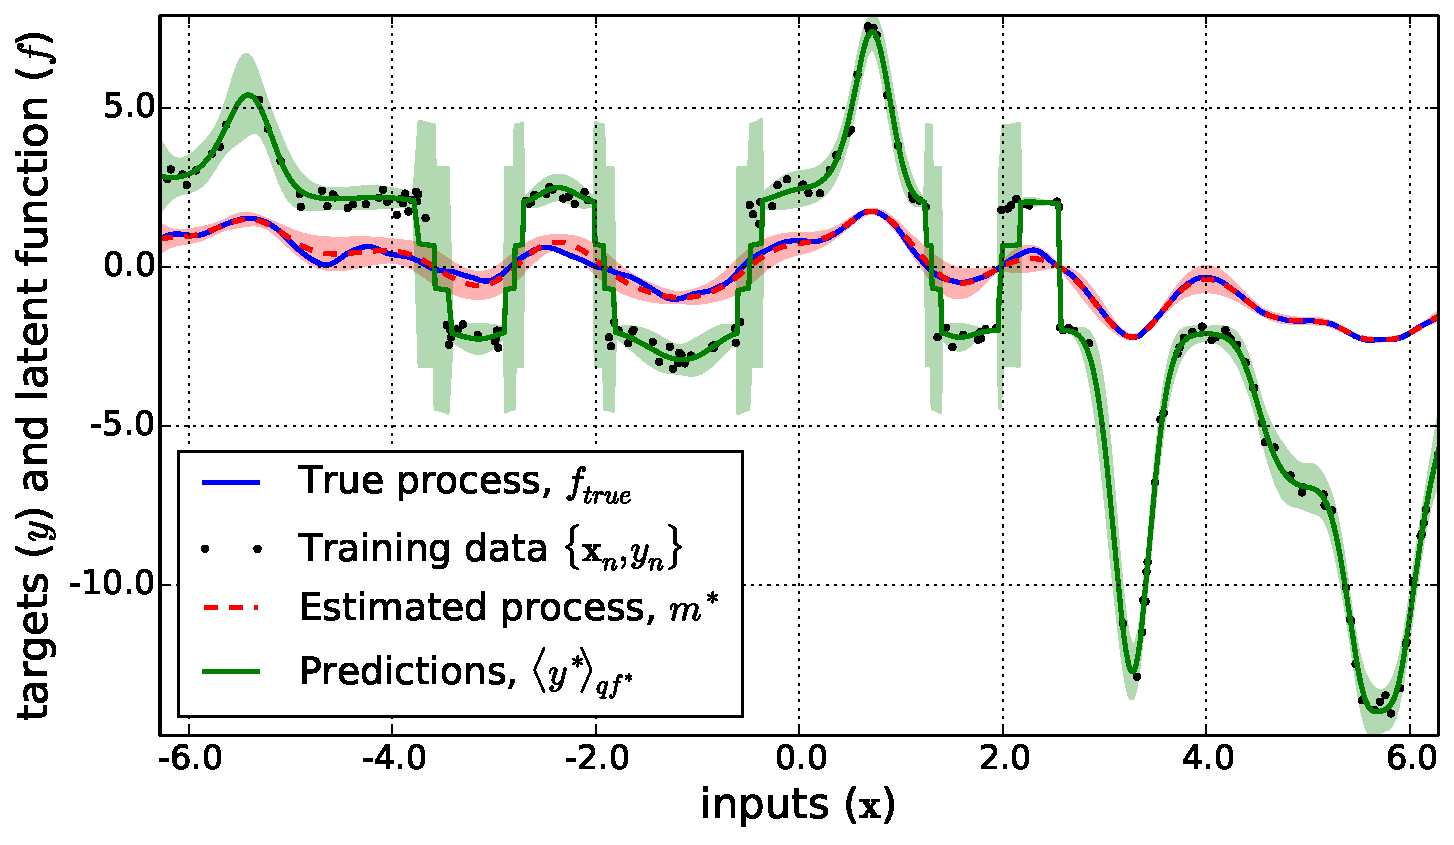
\includegraphics[width=0.5\linewidth]{fig/signdemo}\label{sub:sign}}
    \subfloat[][$\nonlin{\lstate} = \lfloor 5\lstate \rceil$]
        {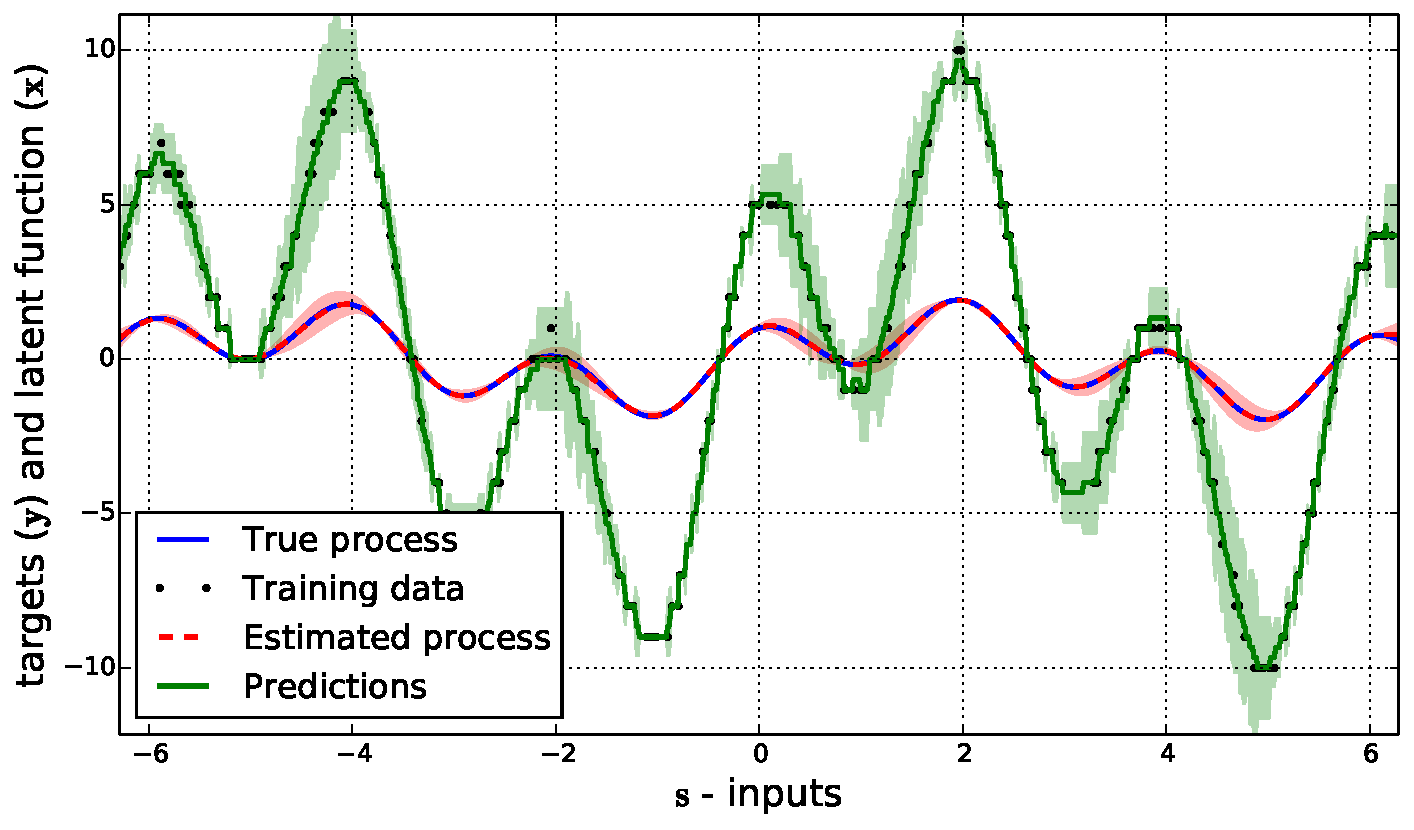
\includegraphics[width=0.5\linewidth]{fig/rounddemo}\label{sub:rnd}}\\
    \subfloat[][MAP trace -- poor hyperparameter values]
        {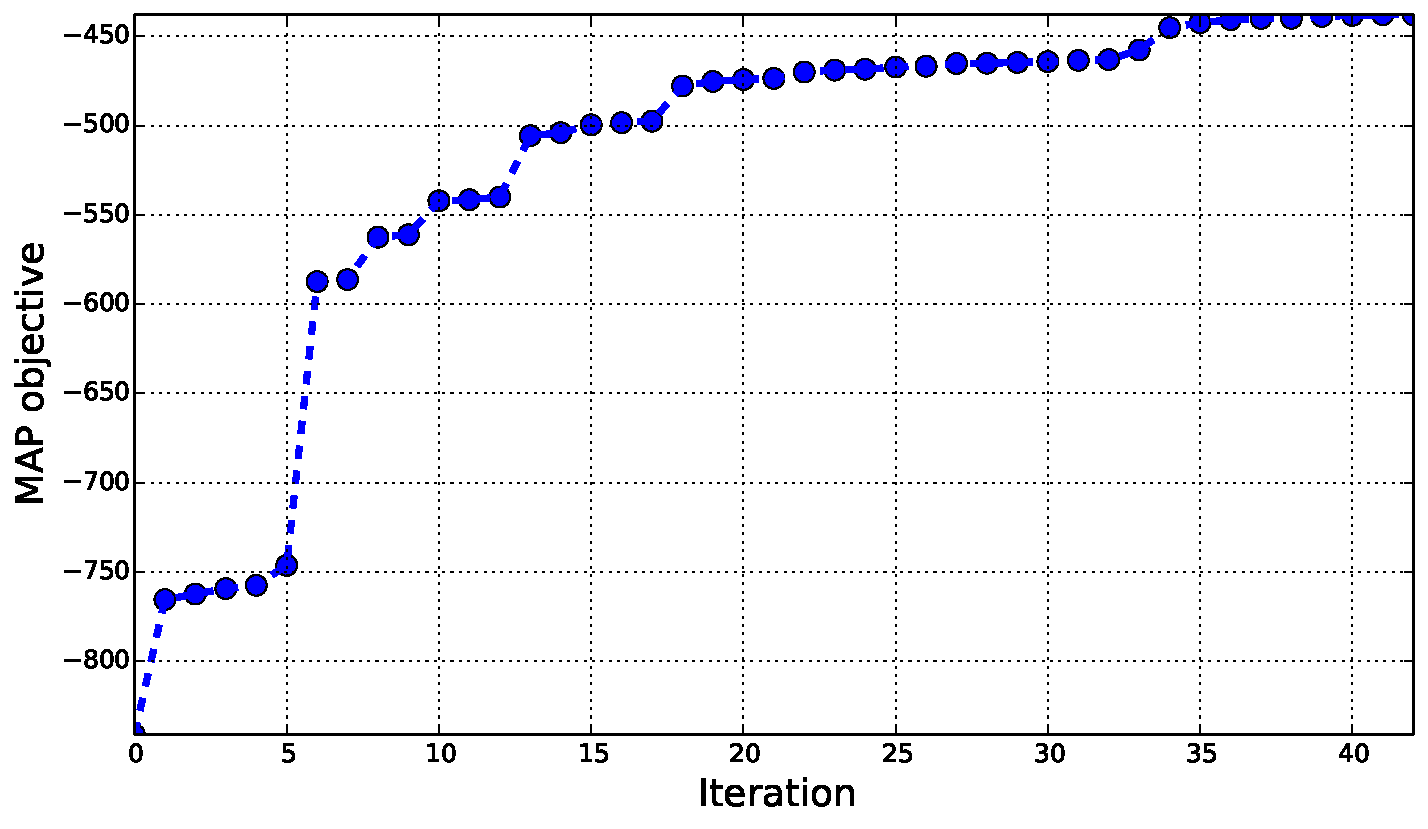
\includegraphics[width=0.5\linewidth]{fig/trace_beg}\label{sub:mapb}}
    \subfloat[][MAP trace -- near optimal hyperprameter values]
        {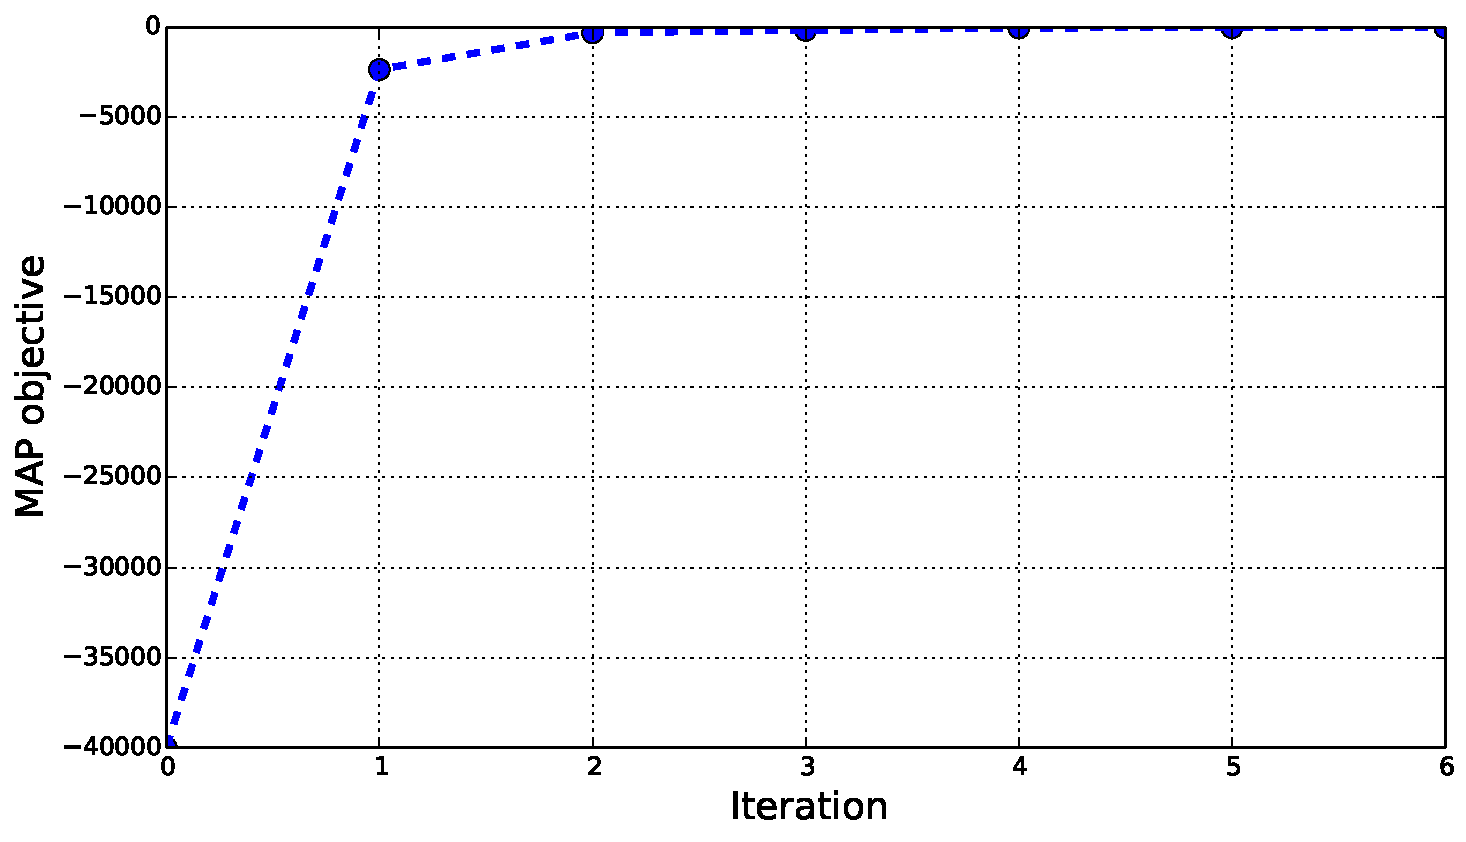
\includegraphics[width=0.5\linewidth]{fig/trace_end}\label{sub:mape}}

    \caption[]{Example of learning the statistically linearised GP with
        non-differentiable nonlinear functions in \subref{sub:sign} and
        \subref{sub:rnd}. In these figures we show the predicitve distribution
        of $\expec{q\lstates}{\obss\test}$ using \eqref{eq:slpred}. Typical
        traces from the MAP objective function used to learn $\pomean$,
        \subref{sub:mapb} is from near the outset of learning the
        hyperparameters, and \subref{sub:mape} is near model convergence --
        both terminated because of `divergence'.}

    \label{fig:learnex}
\end{figure}

\begin{table}[htb]
    \centering
    \small
    \caption[]{Results from running nonlinear likelihood GPs with various
        differentiable nonlinear functions. The true latent function is
        $\lstate_{\text{true}}\!\brac{\inobs} = \sin\!\brac{\inobs} 
            + \cos\!\brac{\pi\inobs}$.}
    \begin{tabular}{r|c| c c c c c c}
        \multirow{2}{*}{$\nonlin{\lstate}$} & \multirow{2}{*}{Algorithm} & 
            \multicolumn{2}{c}{$-\frac{1}{N\test}
                \log\probC{\lstates\test}{\obs}$} &
            \multicolumn{2}{c}{SMSE $\lstates\test$ (\expon{}{-4})} &
            \multicolumn{2}{c}{SMSE $\obss\test$ (\expon{}{-4})} \\
        & & mean & std. & mean & std. & mean & std.\\
        \toprule
        $\lstate$ 
            & Statistical & $-$1.4453 & 0.0601 & 36.471 & 7.309 & -- & -- \\
            & Taylor & 14.2072 & 2.7953 & 54.674 & 8.890 & -- & -- \\
            & \cite{Opper2009} \\
            & Linear & $-$1.2793 & 0.0162 & 40.210 & 7.012 & -- & -- \\
        \midrule
        $\lstate^3 + \lstate^2 + \lstate$ 
            & Statistical & $-$2.1402 & 0.0604 & 27.725 & 6.097 & 36.239 
                & 5.089 \\
            & Taylor & 10.1842 & 1.9443 & 31.094 & 9.193 & 36.991 & 5.869 \\
            & \cite{Opper2009} \\
        \midrule
        $\exp\!\brac{\lstate}$ 
            & Statistical & $-$1.3858 & 0.2320 & 99.405 & 75.756 & 170.07 
                & 27.490 \\
            & Taylor & 15.1875 & 4.0084 & 235.10 & 82.551 & 174.70 & 26.181 \\
            & \cite{Opper2009} \\
        \midrule
        $\sin\!\brac{\lstate}$ 
            & Statistical & $-$0.8892 & 0.1259 & 152.75 & 32.744 & 858.63
                & 104.26 \\
            & Taylor & 20.1577 & 5.9408 & 387.67 & 131.13 & 889.80 & 127.22 \\
            & \cite{Opper2009} \\
        \midrule
        $\tanh\!\brac{2\lstate}$
            & Statistical & $-$0.5903 & 0.1132 & 395.96 & 40.270 & 602.24 
                & 60.622 \\
            & Taylor & 23.7728 & 8.9093 & 894.32 & 523.64 & 606.16 & 64.206 \\
            & \cite{Opper2009} \\
        \bottomrule
    \end{tabular}
\end{table}


\textbf{TODO:} Discuss divergence behaviour of statistical linearisation.


\subsection{Binary Handwritten Digit Classification}

We use the error rate (percent incorrectly predicted labels) and average 
negative log Bernoulli likelihood to asses performance,
\begin{equation}
    - \frac{1}{N\test} \sum^{N\test}_{n} \obss\test_n 
        \log\brac{\pi\test_n}
    + \brac{1-\obss\test_n}\log\brac{1 - \pi\test_n},
\end{equation}
where $\pi\test_n = \expec{}{\prob{\obss\test_n = 1}}$ is predicted from the
classifications algorithms.

A square exponential kernel with amplitude $\sigma_\text{se}$ and length
scale $l_\text{se}$ is used for the Gaussian processes in this experiment.

\begin{table}[htb]
    \centering
    \small
    \caption[]{Binary Gaussian process classifier performance on the USPS
        handwritten-digits dataset for numbers `3' and `5'.}
    \begin{tabular}{r| c c c c}
        Algorithm & Av.\ neg.\ ll. & Error rate (\%) 
            & $\log\!\brac{\sigma_\text{se}}$ & $\log\!\brac{l_\text{se}}$ \\
        \toprule
        GP -- Laplace & 0.11528 & 2.9754 & 2.5855 & 2.5823 \\
        GP -- EP & 0.07522 & 2.4580 & 5.2209 & 2.5315 \\
        SVM (RBF) & 0.08055 & 2.3286 & -- & -- \\
        Logistic Reg. & 0.11995 & 3.6223 & -- & -- \\
        \midrule
        GP -- Statistical & 0.11748 & 2.9754 &  2.8177 & 2.5504 \\
        GP --Taylor & 0.69293 & 42.4321 & 3.1268 & $-$0.1696 \\
        \bottomrule
    \end{tabular}
\end{table}

\section{Conclusion}

\subsubsection*{Acknowledgments}

\subsubsection*{References}
\printbibliography

\end{document}
